\section{ZK Acceleration} \label{sec:zk-acceleration}

The Zero Knowledge calculation process primarily consists of MSM, FFT/IFFT and polynomial evaluation. Given a circuit scale of approximately $2^{25}$, the rough computational consumption ratios are as shown in Figure \ref{fig:time-usage-origin}, ratios will vary for each unique scenario and algorithm.
\begin{figure}[!ht]
    \centering
    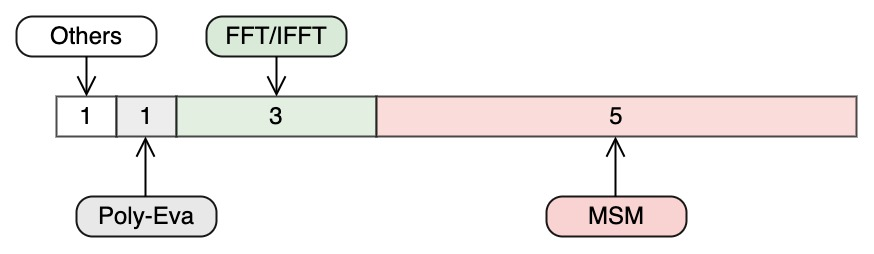
\includegraphics[width=0.8\textwidth]{zk-time-usage.jpg}
    \caption{Consumption ratios of each module of ZK calculation when $n \approx 2^{25}$}
    \label{fig:time-usage-origin}
\end{figure}

Do note that with an increased circuit size, consumption ratio of FFT/IFFT increases as well (because of the better parallelism implementation of MSM than FFT/IFFT), therefore, simply accelerating MSM and FFT/IFFT modules by GPU/FPGA to improve the speed of the prover is limited. We need a ZK algorithm without FFT, where the proportion of FFT/IFFT is so small that it can be ignored, so that the final consumption ratio of each module is close to Figure \ref{fig:time-usage-without-fft}.
\begin{figure}[!ht]
    \centering
    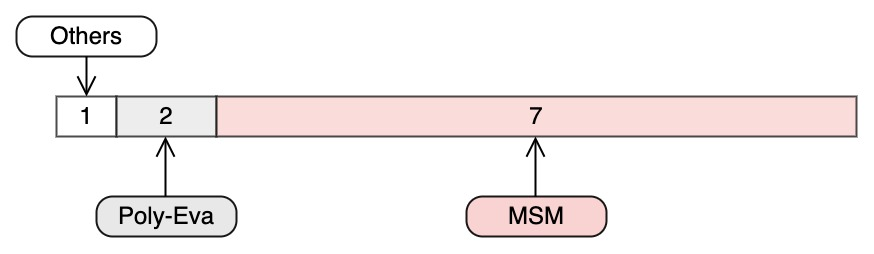
\includegraphics[width=0.8\textwidth]{zk-time-usage-without-fft.jpg}
    \caption{The consumption target ratio of each module of ZK calculation}
    \label{fig:time-usage-without-fft}
\end{figure}

We will introduce additional polynomials to eliminate FFT/IFFT calculations, thus generating additional MSM and polynomial evaluation operations, then using hardware-accelerated designs for MSM and polynomial evaluation operations.

\subsection{MSM of Variable Basis}

Given two vectors $(a_1,a_2,\ldots,a_n)$, $(G_1,G_2,\ldots,G_n)$, where $a_i$ is a field element, and $G_i$ is a point on the elliptic curve, MSM algorithm is to compute the following expressions: $\sum_{i=1}^n a_iG_i$.

\subsubsection{Windowing Method}

Assuming that the bit width of $a_i$ is $b$, we split it into multiple sub-modules with a bit width of $c$. Such sub-modules have a total of $k=\lceil b/c \rceil$, then
\[ a_iG_i = a_{i,0}G_i + 2^ca_{i,1}G_i + \cdots + 2^{(k-1)c}a_{i,k-1}G_i. \]
For all $i$ we have
\begin{align*}
    a_1G_1 &= a_{1,0}G_1 + 2^ca_{1,1}G_1 + \cdots + 2^{(k-1)c}a_{1,k-1}G_1, \\
    a_2G_2 &= a_{2,0}G_2 + 2^ca_{2,1}G_2 + \cdots + 2^{(k-1)c}a_{2,k-1}G_2, \\
    &\cdots \\
    a_nG_n &= a_{n,0}G_n + 2^ca_{n,1}G_n + \cdots + 2^{(k-1)c}a_{n,k-1}G_n.
\end{align*}
So
\[
    \sum_{i=1}^{n} a_iG_i =\sum_{i=1}^{n} \sum_{j=0}^{k-1} a_{i,j} 2^{jc} G_i
    =\sum_{j=0}^{m-1}\left(\sum_{i=1}^{n} a_{i,j} G_i\right) 2^{jc}.
\]
For $a_{i,j} \in [0,2^c)$, we can precompute
\[
    \begin{matrix}
        1G_1 & 2G_1 & \cdots & 2^{c-1}G_1 \\
        1G_2 & 2G_2 & \cdots & 2^{c-1}G_2 \\
        \vdots & \vdots & \ddots & \vdots \\
        1G_n & 2G_n & \cdots & 2^{c-1}G_n
    \end{matrix}
\]

\subsubsection{Endomorphism}

For a cyclic group $\mathbb{G}$ over an elliptic curve $y^2 = x^3 + ax + b$ on a finite field $\mathbb{F}_p$, if one can find such a group endomorphism $\varphi$:
there exists $\alpha, \beta \in \mathbb{F}_p$ such that $\varphi(x, y) = (\alpha x, \beta y)$ holds for all points on $\mathbb{G}$. It is easy to prove that such an automorphism is a multiplicative map, i.e.\ we can find a $\lambda$ such that $\varphi(P) = \lambda P$ holds for all points $P$ on $\mathbb{G}$. This means that when we know the coordinates of a point, we only need to multiply the $x$-coordinate and $y$-coordinate by a number in $\mathbb{F}_p$ to become the coordinates of another point, which can be used for further optimization of the algorithm. If the parameters of the elliptic curve are special, for example, BLS curves can be written as $y^2 = x^3 + b$, and $p \equiv 1 \pmod 3$, taking an element $\alpha$ of order 3 in $\mathbb{F}_p^*$, there exits a corresponding $\lambda$ such that $\lambda (x, y) = (\alpha x, y)$, then the multiplication operation can be optimized as
\begin{align*}
    mP &= (m_1 + m_2\lambda)P \\
    &= m_1P + m_2(\lambda P) \\
    &= m_1P + m_2\varphi(P).
\end{align*}

From \cite{scq03} we can find small $m_1$ and $m_2$ to make the above equation hold, i.e.\ $|m_1|, |m_2| < \sqrt{3 \cdot |\mathbb{G}|}$, which can reduce a multiplication operation of $b$ bits into two multiplication operations of $b/2$ bits. Applied to the windowing method, the number of group operations is reduced to \[ \frac{b}{c}(n+2^c-2) + b-c+\frac{b}{c}-1 \approx \frac{b}{c}(n+2^c). \]
When $n = 10^5$, it can save about 5.5\% of group operations.

\subsection{FPGA Acceleration}

The main flow of MSM calculation in FPGA is shown in Figure \ref{fig:fpga-acceleration}. When performing MSM of a large number of curve points, we mainly use Pippenger's algorithm \cite{pip76} to reduce the calculation of point doubling in MSM calculation process to improve calculation efficiency. Then perform a point addition on the buckets we get from the calculation.

\begin{figure}[!ht]
    \centering
    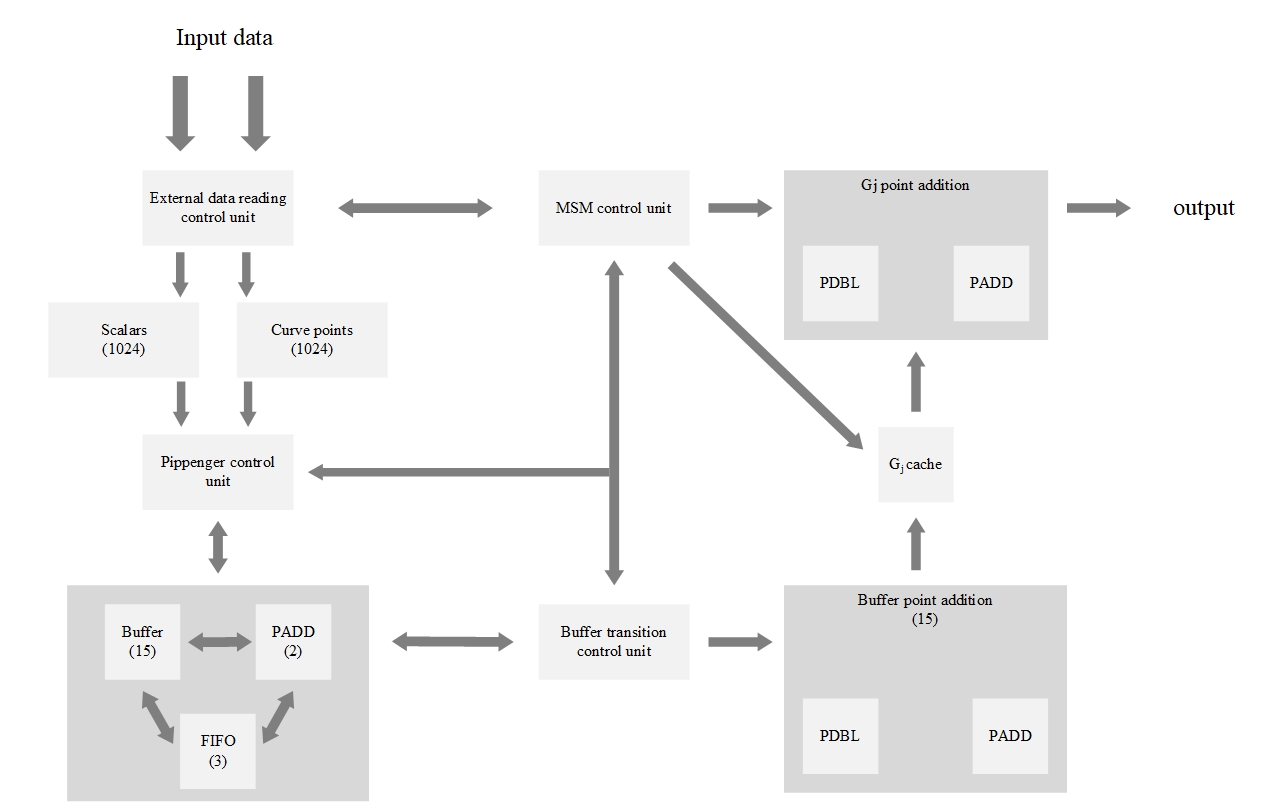
\includegraphics[width=0.8\textwidth]{fpga-acceleration.jpg}
    \caption{FPGA acceleration}
    \label{fig:fpga-acceleration}
\end{figure}

During the whole calculation process, we need a main control logic: MSM control logic, which completes the triggering of the external data reading logic, monitoring the status of the Pippenger control logic, Buffer transition and reading, point addition and point doubling control of the output results of Pippenger's algorithm. This is the brain of MSM.

The core process of the whole calculation is Pippenger's algorithm. In Pippenger's algorithm, firstly, read 1024 scalar values and 1024 curve points from the external memory through the external data reading control logic. Divide the scalar values into 4 bits, and then scan the curve points to complete PADD operation operation. It involves four modules in Pippenger's algorithm: the Pippenger control logic, Buffer, FIFO group and PADD operation. The Pippenger control logic mainly completes the division of sliding windows for scalar values, the cyclic extraction of curve point coordinates and the allocation, control of FIFO reading and writing, and the input and output of PADD. The Buffer buffers the output of PADD operation, while the FIFO group buffers the input of PADD operation.

Due to the limited on-chip memory of FPGA, Pippenger's algorithm can only perform MSM calculations of 1024 points each time. First up, extract the lowest 4 bits of the scalar values and perform point addition of 1024 points. After the addition operations, transfer the cache points in the Buffer, which requires the buffer transition control unit to complete. Secondly, after the point addition operations of 1024 scalars, the next Pippenger of 1024 points needs the Buffer transition control unit to load the Buffer point corresponding to the lowest 4 bits of last time. Then continue the operation, which will also be completed by the Buffer transition control unit.

After the point multiplication operations using Pippenger's algorithm, we need to perform point doubling and point addition operations on the result of the Buffer cache points we get from calculations. Finally, output the operation result of MSM.

